\documentclass[a4paper]{article}

\usepackage[english]{babel}
\usepackage[utf8]{inputenc}
\usepackage{graphicx}
\usepackage{wrapfig}
\usepackage{lipsum}
\usepackage{fullpage}
\usepackage{fancyhdr}
\usepackage{tabularx}

\begin{document}
\pagestyle{fancy}

\renewcommand{\headrulewidth}{0pt}
\lhead{}
\chead{}
\rhead{}
\cfoot{}
\rfoot{}
\lfoot{Copyright © 2014 Stuff Here Inc. --- All rights reserved}

\begin{table}[!th]
\begin{tabular}{l l}
\Large Source: & \Large  sdfawdf awf \\
\\
\Large Language : & \Large  Urdu \\
\\
\Large Level : & \Large BEGINNER \\
\\
\Large Topic : & \Large Culture \\
\end{tabular}
\label{ex:table}
\end{table}
\hrule\hrule\hrule\hrule\vspace{5mm}
\large \textbf{Take a look at the word cloud below and make predictions about the article.}
\begin{center}
	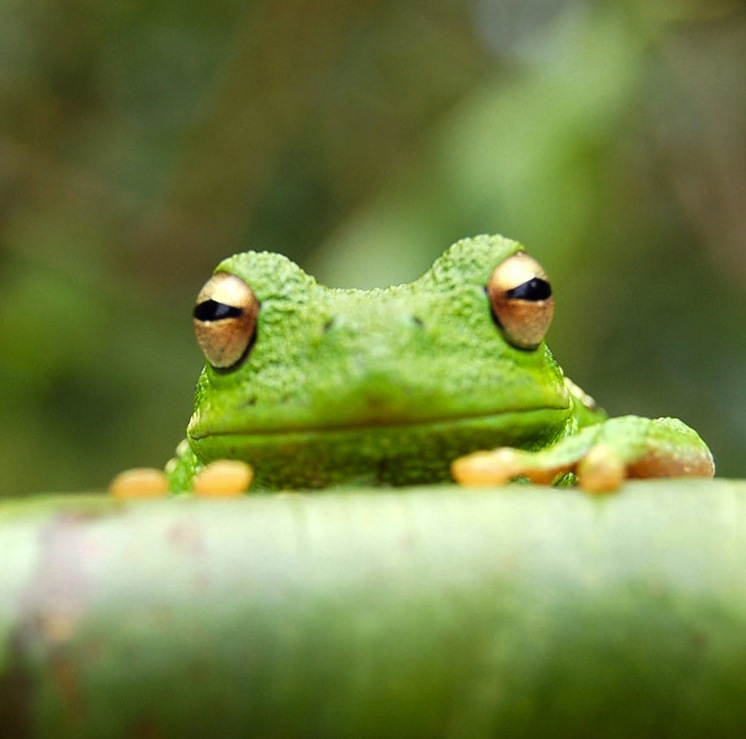
\includegraphics[width=0.48\textwidth]{frog.jpg}
\end{center}


\textbf{Predict the title of the article}\\
\hrule \vspace{5mm}
\hrule \vspace{5mm}
\hrule \vspace{5mm}
\hrule
\pagebreak

\textbf{Sample Concordance Article}
\\ \vspace{5mm}

\raggedright 
\begin{wrapfigure}{l}{0.5\textwidth}
	
\includegraphics[width=0.48\textwidth]{shenron.png}
\end{wrapfigure}
Mocarts ir dzimis Zalcburga, ta laika Zalcburgas arhibiskapijas galvaspilseta, tagadejas Austrijas teritorija, bet tad bija Svetas Romas imperijas sastava. Vina mate bija Anna Marija Mocarte (1720—1778) un tevs Leopolds Mocarts (1719—1787). Abi vecaki sakuma loti uztraucas par Mocarta dzivibu, jo pieci Annas Marijas berni iepriekš jau bija miruši. Mocartam bija ari piecus gadus vecaka masa - Marija Anna (1751—1829), saukta par "Nannerli". Dienu pec piedzimšanas Mocarts tika kristits Sveta Ruperta katedrale. Vinam kristitais vards tika dots latinu valoda - Johanness Hrizostoms Volfgangs Teofils Mocarts (Joannes Chrysostomus Wolfgangus Theophilus Mozart). Mocarts, kad bija pieaudzis, galvenokart sevi deveja par "Volfgangu Amadeju Mocartu" (Wolfgang Amadè Mozart), kaut bija ari varianti.

Mocarta tevs Leopolds Mocarts bija kapelmeistara vietnieks Zalcburgas arhibiskapa galma orkestri, ka ari vijolnieks, ergelnieks un ne seviški nozimigs komponists. Vinš bija ari pieredzejis skolotajs; Mocarta dzimšanas gada vinš publiceja vijolspeles pamatu macibu gramatu, Versuch einer gründlichen Violinschule.

Kad Nannerlei bija septini gadi, Leopolds saka pasniegt vinai klaviernodarbibas. Tris gadus vecais Mocarts acimredzami noskatijas to ar apbrinu: vina masa velak pierakstija, ka šaja vecuma "vinš bieži pavadija daudz laika pie klavierem, izveloties tercas,... un vina prieks paradija, ka tas skaneja labi priekš vina." Nannerle turpinaja: "ceturtaja vina dzives gada tevs, ka rotalu, saka macit vinam nelielus menuetus un klaviergabalus. ... vinš vareja nospelet tos nevai nojami un ar vislielako smalkjutibu, un turoties pareiza tempa. [..] no piecu gadu vecuma vinš jau komponeja nelielus skandarbus, kurus vinš nospeleja savam tevam un tas savukart tos pierakstija." Starp tiem bija Andante (K. 1a) un Allegro C (K. 1b).

Biografs Meinards Solomons atzime, ka, kamer Leopolds ka skolotajs bija loti piekeries saviem berniem, Volfgangs bija motivets gut panakumus pat no ta, ka vina tevs vinu skoloja. Vina pirma patstaviga muzikala kompozicija un vina sakotneja speja spelet vijoli bija gan vina paša darišana, gan lielisks parsteigums Leopoldam. Tevs un dels škiet ir bijuši tuvi; abi iepriekš minetie agrinie notikumi Leopoldu noveda lidz asaram.

Leopolds galu gala beidza komponet, kad vina dela neatkartojamais muzikalais talants kluva acim redzams. vinš bija Volfganga vienigais skolotajs bernibas gados. Tevs jau uzreiz pec Mocarta piedzimšanas ieveroja, ka vinam ir muzika pirksti. Runa, ka Mocarts macejis dziedat vel pirms iemacijies runat. Leopolds saviem berniem tikpat labi ka muziku macija ari valodas, ka ari akademiskos priekšmetus.

Biografs Meinards Solomons atzime, ka, kamer Leopolds ka skolotajs bija loti piekeries saviem berniem, Volfgangs bija motivets gut panakumus pat no ta, ka vina tevs vinu skoloja. Vina pirma patstaviga muzikala kompozicija un vina sakotneja speja spelet vijoli bija gan vina paša darišana, gan lielisks parsteigums Leopoldam. Tevs un dels škiet ir bijuši tuvi; abi iepriekš minetie agrinie notikumi Leopoldu noveda lidz asaram.
Leopolds galu gala beidza komponet, kad vina dela neatkartojamais muzikalais talants kluva acim redzams. vinš bija Volfganga vienigais skolotajs bernibas gados. Tevs jau uzreiz pec Mocarta piedzimšanas ieveroja, ka vinam ir muzika pirksti. Runa, ka Mocarts macejis dziedat vel pirms iemacijies runat. Leopolds saviem berniem tikpat labi ka muziku macija ari valodas, ka ari akademiskos priekšmetus.

Biografs Meinards Solomons atzime, ka, kamer Leopolds ka skolotajs bija loti piekeries saviem berniem, Volfgangs bija motivets gut panakumus pat no ta, ka vina tevs vinu skoloja. Vina pirma patstaviga muzikala kompozicija un vina sakotneja speja spelet vijoli bija gan vina paša darišana, gan lielisks parsteigums Leopoldam. Tevs un dels škiet ir bijuši tuvi; abi iepriekš minetie agrinie notikumi Leopoldu noveda lidz asaram.
Leopolds galu gala beidza komponet, kad vina dela neatkartojamais muzikalais talants kluva acim redzams. vinš bija Volfganga vienigais skolotajs bernibas gados. Tevs jau uzreiz pec Mocarta piedzimšanas ieveroja, ka vinam ir muzika pirksti. Runa, ka Mocarts macejis dziedat vel pirms iemacijies runat. Leopolds saviem berniem tikpat labi ka muziku macija ari valodas, ka ari akademiskos priekšmetus.

Biografs Meinards Solomons atzime, ka, kamer Leopolds ka skolotajs bija loti piekeries saviem berniem, Volfgangs bija motivets gut panakumus pat no ta, ka vina tevs vinu skoloja. Vina pirma patstaviga muzikala kompozicija un vina sakotneja speja spelet vijoli bija gan vina paša darišana, gan lielisks parsteigums Leopoldam. Tevs un dels škiet ir bijuši tuvi; abi iepriekš minetie agrinie notikumi Leopoldu noveda lidz asaram.

Leopolds galu gala beidza komponet, kad vina dela neatkartojamais muzikalais talants kluva acim redzams. vinš bija Volfganga vienigais skolotajs bernibas gados. Tevs jau uzreiz pec Mocarta piedzimšanas ieveroja, ka vinam ir muzika pirksti. Runa, ka Mocarts macejis dziedat vel pirms iemacijies runat. Leopolds saviem berniem tikpat labi ka muziku macija ari valodas, ka ari akademiskos priekšmetus.\\
\pagebreak

\textbf{\Large Read and Answer}
\\
\vspace{5mm}
\
Answer the questions based on the text.
\\
\vspace{5mm}
1. Come up with an alternative title for the text.
\vspace{5mm}
\\
\hrule \vspace{5mm}
\hrule \vspace{5mm}
\hrule \vspace{5mm}
\hrule \vspace{5mm}
\vspace{5mm}
2. What happened (in the story/before/after)
\vspace{5mm}
\\
\hrule \vspace{5mm}
\hrule \vspace{5mm}
\hrule \vspace{5mm}
\hrule \vspace{5mm}
\vspace{5mm}
3. Who said...?
\vspace{5mm}
\\
\hrule \vspace{5mm}
\hrule \vspace{5mm}
\hrule \vspace{5mm}
\hrule \vspace{5mm}
\vspace{5mm}
\pagebreak
\Large \textbf{Fill in the Blanks}
\\ \vspace{5mm}
\normalsize \textbf{Write the word that best completes each blank. Select from the word bank below}\\
\vspace{5mm}
\raggedright Mocarts ir dzimis Zalcburga, ta laika Zalcburgas arhibiskapijas galvaspilseta, tagadejas Austrijas teritorija, bet tad bija Svetas Romas imperijas sastava. Vina mate bija Anna Marija Mocarte (1720—1778) un tevs Leopolds Mocarts (1719—1787). Abi vecaki sakuma \_\_\_\_\_\_ uztraucas par Mocarta dzivibu, jo pieci Annas Marijas berni iepriekš jau bija miruši. Mocartam bija ari piecus gadus vecaka masa - Marija Anna (1751—1829), saukta par "Nannerli". Dienu pec piedzimšanas Mocarts tika kristits Sveta Ruperta katedrale. Vinam kristitais vards tika dots latinu valoda - Johanness Hrizostoms Volfgangs Teofils Mocarts (Joannes Chrysostomus Wolfgangus Theophilus Mozart). Mocarts, kad bija pieaudzis, galvenokart sevi deveja par "Volfgangu Amadeju Mocartu" (\_\_\_\_\_\_), kaut bija ari varianti.

Mocarta tevs Leopolds Mocarts bija kapelmeistara vietnieks Zalcburgas arhibiskapa galma orkestri, ka ari vijolnieks, ergelnieks un ne seviški nozimigs komponists. Vinš bija ari pieredzejis skolotajs; Mocarta dzimšanas gada vinš publiceja vijolspeles pamatu macibu gramatu, Versuch einer gründlichen Violinschule.

Kad Nannerlei bija septini gadi, \_\_\_\_\_\_ saka pasniegt vinai klaviernodarbibas. Tris gadus vecais Mocarts acimredzami noskatijas to ar apbrinu: vina masa velak pierakstija, ka šaja vecuma "vinš bieži pavadija daudz laika pie klavierem, izveloties tercas,... un vina prieks paradija, ka tas skaneja labi priekš vina." Nannerle turpinaja: "ceturtaja vina dzives gada tevs, ka rotalu, saka macit vinam nelielus menuetus un klaviergabalus. ... vinš vareja nospelet tos nevai nojami un ar vislielako smalkjutibu, un turoties pareiza tempa. [..] no piecu gadu vecuma vinš jau komponeja nelielus skandarbus, kurus vinš nospeleja savam tevam un tas savukart tos pierakstija." Starp tiem bija Andante (K. 1a) un Allegro C (K. 1b).

Biografs Meinards Solomons atzime, ka, kamer Leopolds ka skolotajs bija loti piekeries saviem berniem, Volfgangs bija motivets gut panakumus pat no ta, ka vina tevs vinu skoloja. Vina pirma patstaviga muzikala kompozicija un vina sakotneja speja spelet vijoli bija gan vina paša darišana, gan lielisks parsteigums Leopoldam. Tevs un dels škiet ir bijuši tuvi; abi iepriekš minetie agrinie notikumi Leopoldu noveda lidz asaram.

Leopolds galu gala beidza komponet, kad vina dela neatkartojamais muzikalais talants kluva acim redzams. vinš bija Volfganga vienigais skolotajs bernibas gados. Tevs jau uzreiz pec Mocarta piedzimšanas ieveroja, ka vinam ir muzika pirksti. Runa, ka Mocarts macejis dziedat vel pirms iemacijies runat. Leopolds saviem berniem tikpat labi ka muziku macija ari valodas, ka ari akademiskos priekšmetus.

Biografs Meinards Solomons atzime, ka, \_\_\_\_\_\_ Leopolds ka skolotajs bija loti piekeries saviem berniem, Volfgangs bija motivets gut panakumus pat no ta, ka vina tevs vinu skoloja. Vina pirma patstaviga muzikala kompozicija un vina sakotneja speja spelet vijoli bija gan vina paša darišana, gan lielisks parsteigums Leopoldam. Tevs un dels škiet ir bijuši tuvi; abi iepriekš minetie agrinie notikumi Leopoldu noveda lidz asaram.
Leopolds galu gala beidza komponet, kad vina dela neatkartojamais muzikalais talants kluva acim redzams. vinš bija Volfganga vienigais skolotajs bernibas gados. Tevs jau uzreiz pec Mocarta piedzimšanas ieveroja, ka vinam ir muzika pirksti. Runa, ka Mocarts macejis dziedat vel pirms iemacijies runat. Leopolds saviem berniem tikpat labi ka muziku macija ari valodas, ka ari akademiskos priekšmetus.

Biografs Meinards Solomons atzime, ka, kamer Leopolds ka skolotajs bija loti piekeries saviem berniem, Volfgangs bija motivets gut panakumus pat no ta, ka vina tevs vinu skoloja. Vina pirma patstaviga muzikala kompozicija un vina sakotneja speja spelet vijoli bija gan vina paša darišana, gan lielisks parsteigums Leopoldam. Tevs un dels škiet ir bijuši tuvi; abi iepriekš minetie agrinie notikumi Leopoldu noveda lidz asaram.
Leopolds galu gala beidza komponet, kad vina dela neatkartojamais muzikalais talants kluva acim redzams. vinš bija Volfganga vienigais skolotajs bernibas gados. Tevs jau uzreiz pec Mocarta piedzimšanas ieveroja, ka vinam ir muzika pirksti. Runa, ka Mocarts macejis dziedat vel pirms iemacijies runat. Leopolds saviem berniem tikpat labi ka muziku macija ari valodas, ka ari akademiskos priekšmetus.

Biografs Meinards Solomons atzime, ka, kamer Leopolds ka skolotajs bija loti piekeries saviem berniem, Volfgangs bija motivets gut panakumus pat no ta, ka vina tevs vinu skoloja. Vina pirma patstaviga muzikala kompozicija un vina sakotneja speja spelet vijoli bija gan vina paša darišana, gan lielisks parsteigums Leopoldam. Tevs un dels škiet ir bijuši tuvi; abi iepriekš minetie agrinie notikumi Leopoldu noveda lidz asaram.

Leopolds galu gala beidza komponet, kad vina dela neatkartojamais muzikalais talants kluva acim redzams. vinš bija Volfganga vienigais skolotajs bernibas gados. Tevs jau uzreiz pec Mocarta piedzimšanas ieveroja, ka vinam ir muzika pirksti. Runa, ka Mocarts macejis dziedat vel pirms iemacijies runat. Leopolds saviem berniem tikpat labi ka muziku macija ari valodas, ka ari akademiskos priekšmetus.\\
\vspace{5mm}
\vspace{5mm}
\textbf{Word Bank}\\
\begin{table}[!th]
\begin{tabularx}{\textwidth}{X X X}
loti & kamer & Leopolds\\
 & & \\
Wolfgang Amadè Mozart
\\
\vspace{5mm}
\end{tabularx}
\end{table}

\pagebreak
\Large \textbf{Matching} \\
\vspace{5mm}
\normalsize \textbf{ Match the following words to their definitions}
\begin{table}[!th]
\begin{tabularx}{\textwidth}{X X}
\underline{Vocabulary} & \underline{Translation} \\
& \\
1) galvaspilsētā & 1) Baptized \\
& \\
2) uztraucās & 2) worried \\
& \\
3) Mocarts & 3) Mozart \\
& \\
4) kristīts & 4) older\\
& \\
5) vecāka & 5) capital \\

\end{tabularx}
\end{table}


\Large \textbf{Multiple Choice} \\
\vspace{5mm}
\normalsize \textbf{Select the best answer} \\


\begin{table}[!th]
\begin{tabularx}{\textwidth}{X X X}
& \underline{galvaspilsētā} & \\
a. older & & b. Baptized \\
& \\
c. capital & & d. Mozart \\

& \\
& \\

& \underline{uztraucās} & \\
a. capital & & b. worried \\
& \\
c. Mozart & & d. older \\

& \\
& \\

& \underline{Mocarts} & \\
a. capital & & b. worried \\
& \\
c. Mozart & & d. Baptized\\

& \\
& \\

& \underline{kristīts} & \\
a. capital & & b. Baptized\\
& \\
c. older & & d. Mozart\\

& \\
& \\

& \underline{vecāka Black a Borla Ehnmve Eekjfp so} & \\
a. Baptized & & b. worried\\
& \\
c. Mozart & & d. older\\
\end{tabularx}
\end{table}

\raggedright
\pagebreak

\Huge \textbf{Answer Key}
\\ \vspace{5mm}
\Large \textbf{Fill in the Blanks}
\\ \vspace{5mm}

\raggedright Mocarts ir dzimis Zalcburga, ta laika Zalcburgas arhibiskapijas galvaspilseta, tagadejas Austrijas teritorija, bet tad bija Svetas Romas imperijas sastava. Vina mate bija Anna Marija Mocarte (1720—1778) un tevs Leopolds Mocarts (1719—1787). Abi vecaki sakuma \underline{loti} uztraucas par Mocarta dzivibu, jo pieci Annas Marijas berni iepriekš jau bija miruši. Mocartam bija ari piecus gadus vecaka masa - Marija Anna (1751—1829), saukta par "Nannerli". Dienu pec piedzimšanas Mocarts tika kristits Sveta Ruperta katedrale. Vinam kristitais vards tika dots latinu valoda - Johanness Hrizostoms Volfgangs Teofils Mocarts (Joannes Chrysostomus Wolfgangus Theophilus Mozart). Mocarts, kad bija pieaudzis, galvenokart sevi deveja par "Volfgangu Amadeju Mocartu" (\underline{Wolfgang Amadè Mozart}), kaut bija ari varianti.

Mocarta tevs Leopolds Mocarts bija kapelmeistara vietnieks Zalcburgas arhibiskapa galma orkestri, ka ari vijolnieks, ergelnieks un ne seviški nozimigs komponists. Vinš bija ari pieredzejis skolotajs; Mocarta dzimšanas gada vinš publiceja vijolspeles pamatu macibu gramatu, Versuch einer gründlichen Violinschule.

Kad Nannerlei bija septini gadi, \underline{Leopolds} saka pasniegt vinai klaviernodarbibas. Tris gadus vecais Mocarts acimredzami noskatijas to ar apbrinu: vina masa velak pierakstija, ka šaja vecuma "vinš bieži pavadija daudz laika pie klavierem, izveloties tercas,... un vina prieks paradija, ka tas skaneja labi priekš vina." Nannerle turpinaja: "ceturtaja vina dzives gada tevs, ka rotalu, saka macit vinam nelielus menuetus un klaviergabalus. ... vinš vareja nospelet tos nevai nojami un ar vislielako smalkjutibu, un turoties pareiza tempa. [..] no piecu gadu vecuma vinš jau komponeja nelielus skandarbus, kurus vinš nospeleja savam tevam un tas savukart tos pierakstija." Starp tiem bija Andante (K. 1a) un Allegro C (K. 1b).

Biografs Meinards Solomons atzime, ka, kamer Leopolds ka skolotajs bija loti piekeries saviem berniem, Volfgangs bija motivets gut panakumus pat no ta, ka vina tevs vinu skoloja. Vina pirma patstaviga muzikala kompozicija un vina sakotneja speja spelet vijoli bija gan vina paša darišana, gan lielisks parsteigums Leopoldam. Tevs un dels škiet ir bijuši tuvi; abi iepriekš minetie agrinie notikumi Leopoldu noveda lidz asaram.

Leopolds galu gala beidza komponet, kad vina dela neatkartojamais muzikalais talants kluva acim redzams. vinš bija Volfganga vienigais skolotajs bernibas gados. Tevs jau uzreiz pec Mocarta piedzimšanas ieveroja, ka vinam ir muzika pirksti. Runa, ka Mocarts macejis dziedat vel pirms iemacijies runat. Leopolds saviem berniem tikpat labi ka muziku macija ari valodas, ka ari akademiskos priekšmetus.

Biografs Meinards Solomons atzime, ka, \underline{kamer} Leopolds ka skolotajs bija loti piekeries saviem berniem, Volfgangs bija motivets gut panakumus pat no ta, ka vina tevs vinu skoloja. Vina pirma patstaviga muzikala kompozicija un vina sakotneja speja spelet vijoli bija gan vina paša darišana, gan lielisks parsteigums Leopoldam. Tevs un dels škiet ir bijuši tuvi; abi iepriekš minetie agrinie notikumi Leopoldu noveda lidz asaram.
Leopolds galu gala beidza komponet, kad vina dela neatkartojamais muzikalais talants kluva acim redzams. vinš bija Volfganga vienigais skolotajs bernibas gados. Tevs jau uzreiz pec Mocarta piedzimšanas ieveroja, ka vinam ir muzika pirksti. Runa, ka Mocarts macejis dziedat vel pirms iemacijies runat. Leopolds saviem berniem tikpat labi ka muziku macija ari valodas, ka ari akademiskos priekšmetus.

Biografs Meinards Solomons atzime, ka, kamer Leopolds ka skolotajs bija loti piekeries saviem berniem, Volfgangs bija motivets gut panakumus pat no ta, ka vina tevs vinu skoloja. Vina pirma patstaviga muzikala kompozicija un vina sakotneja speja spelet vijoli bija gan vina paša darišana, gan lielisks parsteigums Leopoldam. Tevs un dels škiet ir bijuši tuvi; abi iepriekš minetie agrinie notikumi Leopoldu noveda lidz asaram.
Leopolds galu gala beidza komponet, kad vina dela neatkartojamais muzikalais talants kluva acim redzams. vinš bija Volfganga vienigais skolotajs bernibas gados. Tevs jau uzreiz pec Mocarta piedzimšanas ieveroja, ka vinam ir muzika pirksti. Runa, ka Mocarts macejis dziedat vel pirms iemacijies runat. Leopolds saviem berniem tikpat labi ka muziku macija ari valodas, ka ari akademiskos priekšmetus.

Biografs Meinards Solomons atzime, ka, kamer Leopolds ka skolotajs bija loti piekeries saviem berniem, Volfgangs bija motivets gut panakumus pat no ta, ka vina tevs vinu skoloja. Vina pirma patstaviga muzikala kompozicija un vina sakotneja speja spelet vijoli bija gan vina paša darišana, gan lielisks parsteigums Leopoldam. Tevs un dels škiet ir bijuši tuvi; abi iepriekš minetie agrinie notikumi Leopoldu noveda lidz asaram.

Leopolds galu gala beidza komponet, kad vina dela neatkartojamais muzikalais talants kluva acim redzams. vinš bija Volfganga vienigais skolotajs bernibas gados. Tevs jau uzreiz pec Mocarta piedzimšanas ieveroja, ka vinam ir muzika pirksti. Runa, ka Mocarts macejis dziedat vel pirms iemacijies runat. Leopolds saviem berniem tikpat labi ka muziku macija ari valodas, ka ari akademiskos priekšmetus.\\

\vspace{5mm}

\Large \textbf{Matching} \\
\begin{table}[!th]
\begin{tabularx}{\textwidth}{c c c}
\underline{Vocabulary} & & \underline{Translation} \\
& \\
1) galvaspilsētā & --- & 5) capital  \\
& \\
2) uztraucās & --- & 2) worried \\
& \\
3) Mocarts & --- & 3) Mozart \\
& \\
4) kristīts & --- & 1) Baptized\\
& \\
5) vecāka & --- & 4) older \\
\end{tabularx}
\end{table}

\Large \textbf{Multiple Choice} \\

\begin{table}[!th]
\begin{tabularx}{\textwidth}{c c c}
\underline{Vocabulary} & & \underline{Translation} \\

& \\

galvaspilsētā & --- & c. capital \\

& \\

uztraucās & --- & b. worried \\

& \\

Mocarts & --- & c. Mozart \\

& \\

kristīts & --- & b. Baptized\\

& \\

vecāka & --- & d. older\\
\end{tabularx}
\end{table}


\end{document}
